\chapter{Bildvorverarbeitung \dcfirstauthorshort}
\label{cha:bildvorverarbeitung}

Bevor nach der Aufnahme des Bildes nach Linien gesucht werden kann, muss das Bild entzerrt, gefiltert und binarisiert werden. 

\section{Bildentzerrung}

Der große Vorteil des Fischaugenobjektivs ist es, Bereiche in größerer Entfernung in alle Richtungen  wahrnehmen zu können. Jedoch ist es gerade für die Approximation der Fahrbahnmarkierungen zur Erstellung einer Weltkarte und der Regelung des Autos sinnvoll, dessen Verzerrung zu rektifizieren. Dazu wurde sich in MATLAB wie in~\ref{sec:kameramodell} beschrieben der \gls{acr:ocamcalib}-Toolbox bedient. Zuvor erfolgt außerdem eine Umwandlung in ein Graustufenbild, da wir die Farbinformation der Rohdaten nicht mit verarbeiten und sowohl die Toolbox als auch die Filter nur mit Schwarz-Weiß-Bildern, also einer Matrix deren Einträge die Helligkeitswerte der Pixel darstellt, arbeiten können. 

% Das ver- und entzerrte Bild nebeneinander
\begin{figure}[ht] % [htb]
  \centering
  \subfloat[][]{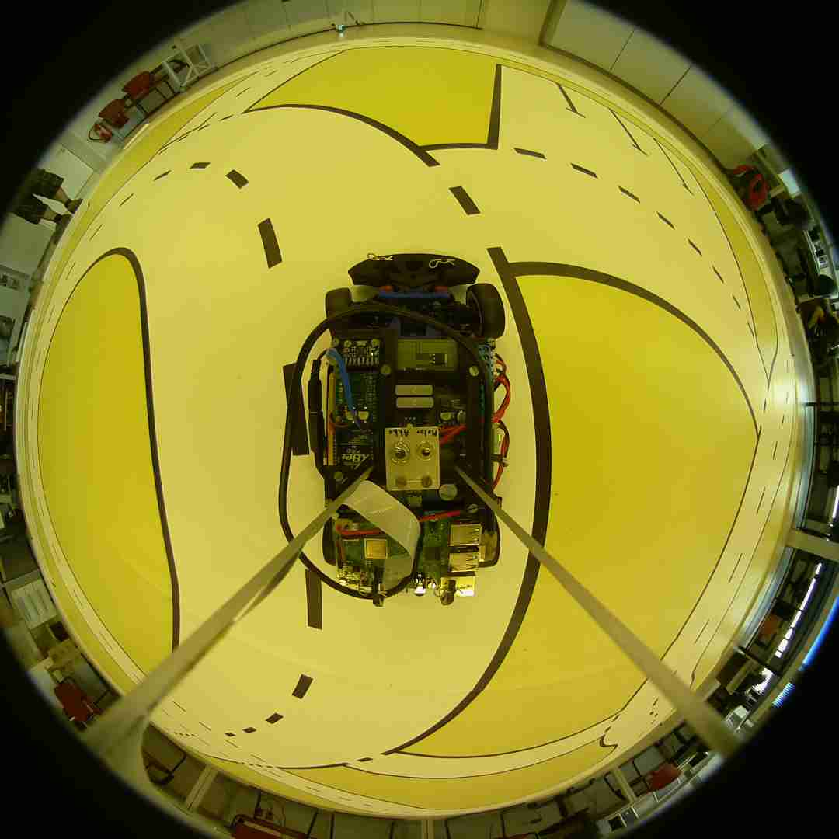
\includegraphics[width=0.45\textwidth]{bildvorverarbeitung_fischauge.png}}
  \qquad
  \subfloat[][]{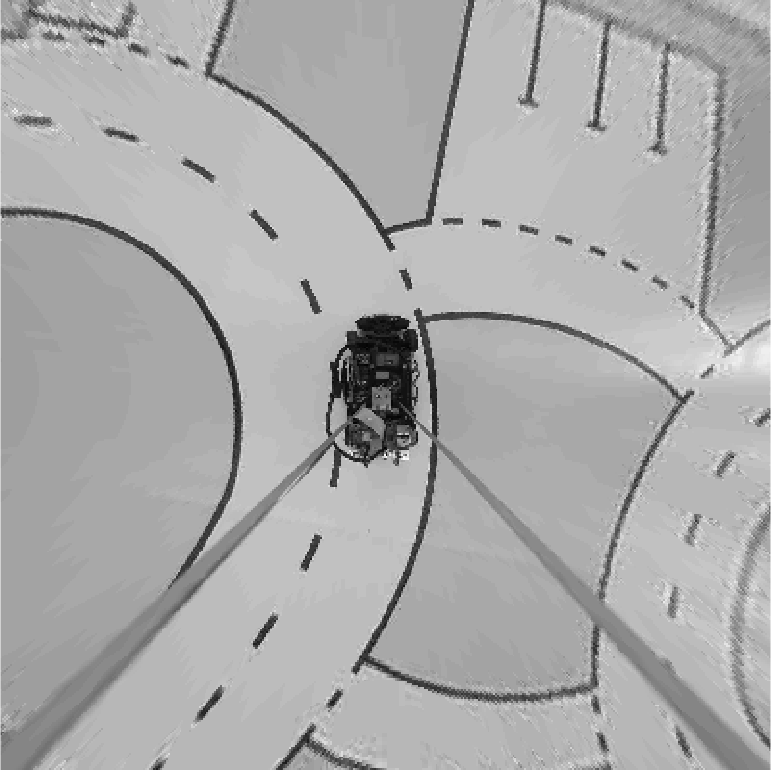
\includegraphics[width=0.45\textwidth]{bildvorverarbeitung_entzerrt.png}}
%  \includegraphics[width=0.9\textwidth]{bildvorverarbeitung_entzerren.png}
  \caption{verzerrtes Rohbild (a) und entzerrtes Graustufenbild (b) einer Momentaufnahme im Parcours}
\label{fig:bildvorverarbeitung_entzerren}
\end{figure} 

In~\ref{fig:bildvorverarbeitung_entzerren} ist ein Bild original (links) und nach der Entzerrung (rechts) zu sehen. Im entzerrten Bild fällt auf, dass zum Rand die Auflösung durch dessen Transformation zunehmend schlechter wird. 
Daher haben wir den Bildausschnitt bis auf die nach der Filterung akzeptabel erkennbaren Linien begrenzt.

\section{Filterung}
\label{sec:bildvorverarbeitung:filterung}
Die Aufnahme soll nun wie in~\ref{sec:filter} beschrieben gefiltert werden, damit die Kanten (sprich: steile Übergänge von hellen zu dunklen Pixeln oder andersherum) hervorgehoben werden. Monotone Bildbereiche sollen dunkel bleiben. Unter Durchführung einer Kantendetektion auf dem entzerrten Bild erhielte man sehr viele Treffer, da durch sensorbedingtes Bildrauschen den Kantendetektor ansprechende Störungen enthalten sind. Das in Abbildung ~\ref{fig:bildvorverarbeitung_filtern} (a) dargestellte Filterergebnis wurde mit einem \gls{acr:log}-Filter erzielt. Dieser vereint mit der gaußschen Glättung und dem Laplace-Operator die Ausführung zweier Filter. Wie in Abschnitt~\ref{ssec:laplaceFilter} erklärt, stellen Kanten in der Filterantwort die Nulldurchgänge zwischen den positiven und negativen Peaks dar. Da das gefilterte Bild keine Pixelwerte kleiner Null zugewiesen bekommt, sind nur deren stark positiven Anstiegsänderungen (2. Ableitung \( > 0\)) in~\ref{fig:bildvorverarbeitung_filtern} (a) sichtbar. Im Allgemeinen treten an einer Linie zwei Kanten auf. Jedoch lassen sich mit entsprechend eingestellten Parameterwerten die zwei an jeder Fahrbahnmarkierung entstandenen positiven Peaks zu einer sichtbaren, die Fahrbahnbegrenzung repräsentierenden, hellen Linie verwischen. 

Um wertvolle Rechenzeit bei der aufwändigen Filterung einzusparen, werden das Bild mit je einem eindimensionalen Filter in \( {\gls{x}}^{\gls{lat:BildKOS}} \)- und \( {\gls{y}}^{\gls{lat:BildKOS}} \)-Richtung verarbeitet und anschließend die Filterergebnisse addiert. Diese Alternative zu der in~\ref{sec:filter} beschriebenen Separierbarkeit hat einen deutlich schnelleren Funktionsablauf ermöglicht. Erstaunlicherweise ist die Qualität des gefilterten Bildes sehr gut, sodass die Weiterverarbeitung verlässliche Informationen liefert.


% Das gefilterte und binarisierte Bild nebeneinander
\begin{figure}[H] % [htb]
  \centering
  \subfloat[][]{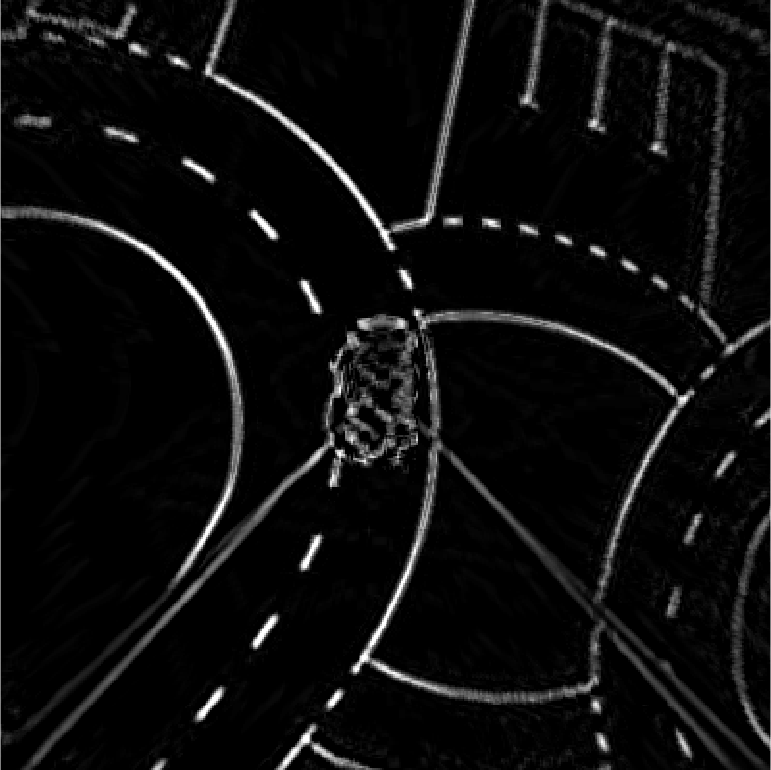
\includegraphics[width=0.45\textwidth]{bildvorverarbeitung_gefiltert.png}}
  \qquad
  \subfloat[][]{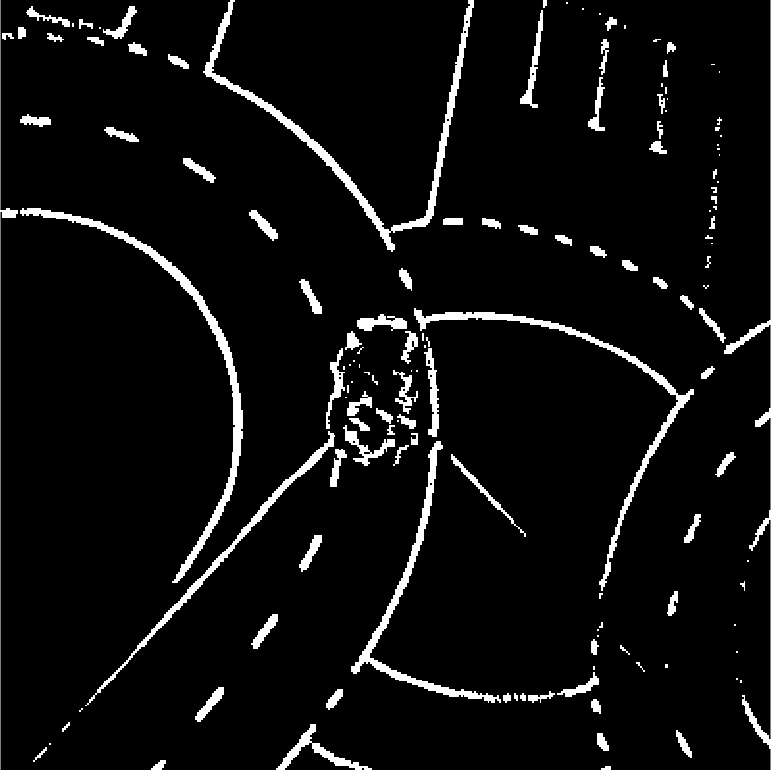
\includegraphics[width=0.45\textwidth]{bildvorverarbeitung_binarisiert.png}}
  \caption{gefiltertes (a) und anschließend binarisiertes Bild (b) einer Momentaufnahme im Parcours}
\label{fig:bildvorverarbeitung_filtern}
\end{figure} 

\section{Binarisierung}

Der Schwellwert, welcher entscheidet, ob ein Pixel im binarisierten Bild den Wert \glqq \(0\)\grqq{} oder\glqq \(1\)\grqq{} erhält, wurde fest als Parameter eingestellt. Alle weiteren Bildverarbeitungsalgorithmen ziehen das binarisierte oder gefilterte Bild als Grundlage ihrer Berechnungen heran.